\section{Methods}
The Ferienakademie uses many methods to attain the attention of students. In this section we want to present some of them. Furthermore, we want to take a look at how they are applied.
\subsection{Courses}
Of course, the main method are the courses themselves. As already stated, right now there exists a wide variety of courses from possibly very different fields-- informatics, mathematics, medical engineering, psychology, philosophy, etc. The group size usually varies between 10-20 students. 

The typical structure of the course is the following: Suitable to the main topic of the course, students prepare a talk for a specific topic before the start of Ferienakademie. 

Some courses also offer a project during the summer school. While students still might prepare a talk, they work on specific projects in groups during their time in Sarntal. In 2015, for example, course 2 developed apps for iOS to enhance the quality of life, while course 5 created a game based on multiphysics simulation using the Xbox Kinect. 

In both cases, the small size of the group, the close interaction with the corresponding professors and the motivation of each participating student (and also the non-existent pressure of grading) creates a special atmosphere which leads to exciting discussions, not only during the course itself. (Rumours exist that whole game ideas where developed, discarded and reinvented during hikes.)

Examples of both types of courses are shown in \autoref{fig:presentation} and \autoref{fig:project}.
\begin{figure}[ht]%
 	\begin{center}%
 		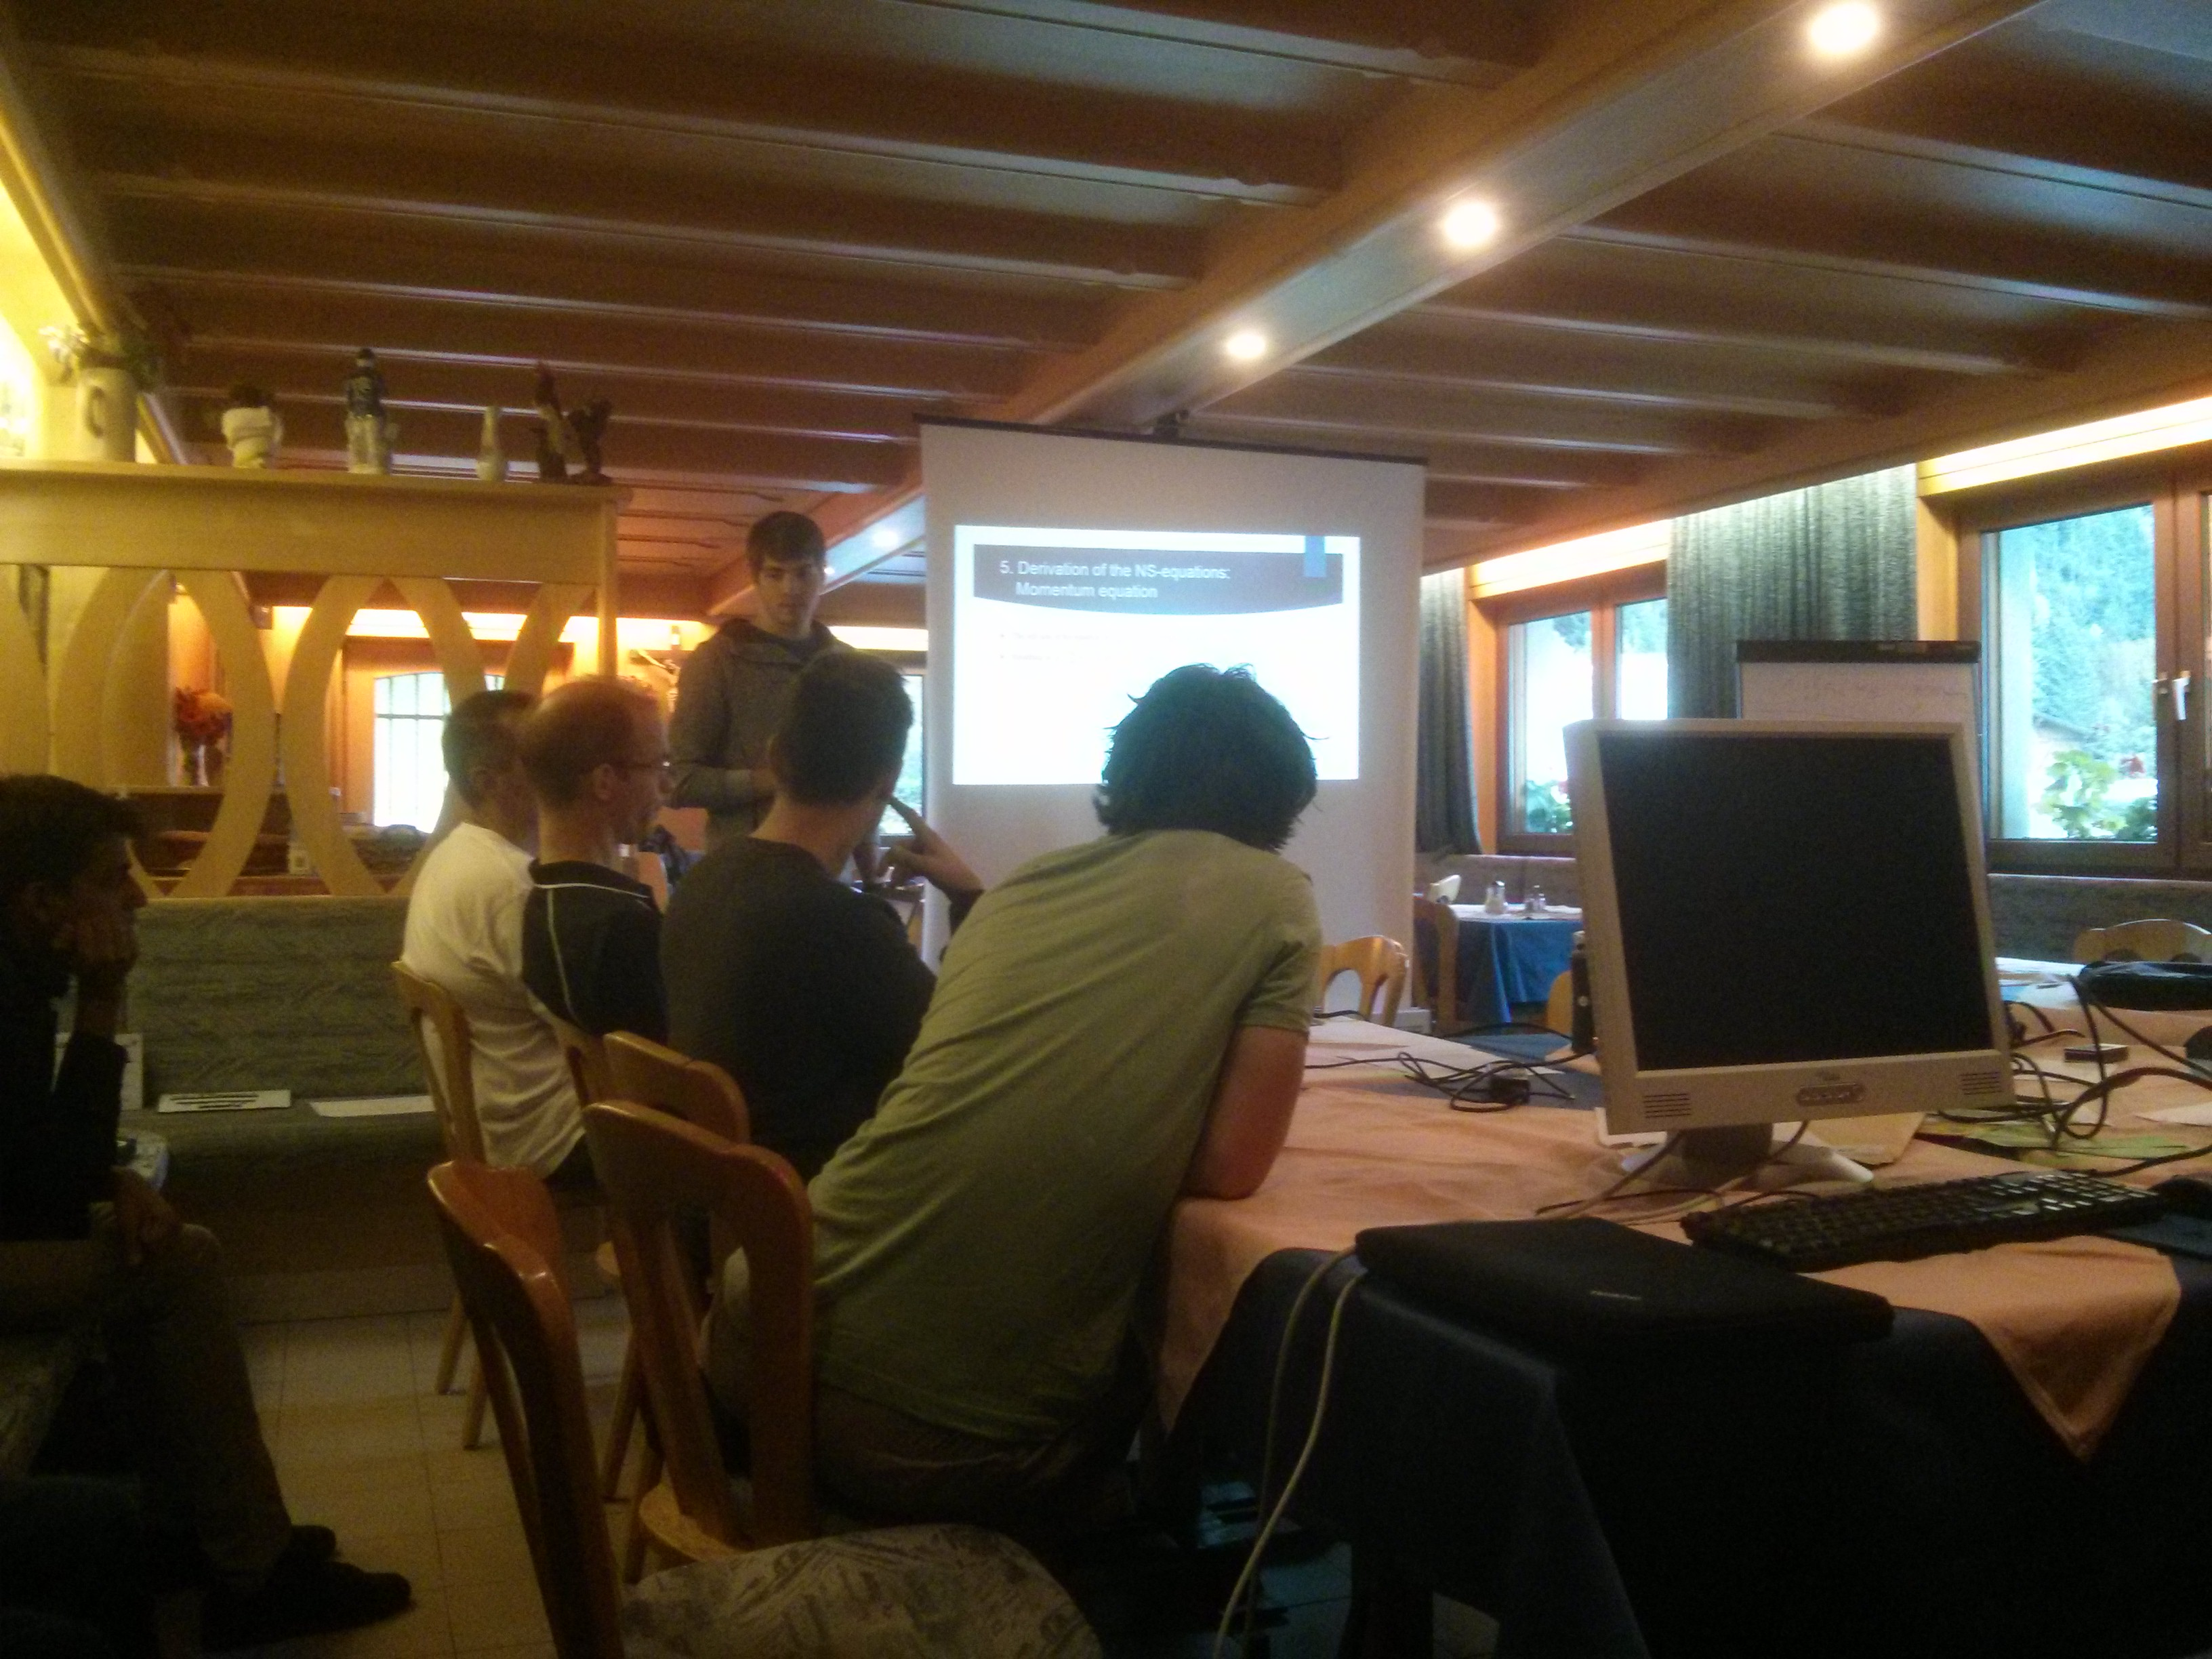
\includegraphics[scale=0.048]{img/Presentation.jpg}%
 		\caption{Presentation in a course.}\label{fig:presentation}%
 	\end{center}%
\end{figure}
\begin{figure}[ht]%
 	\begin{center}%
 		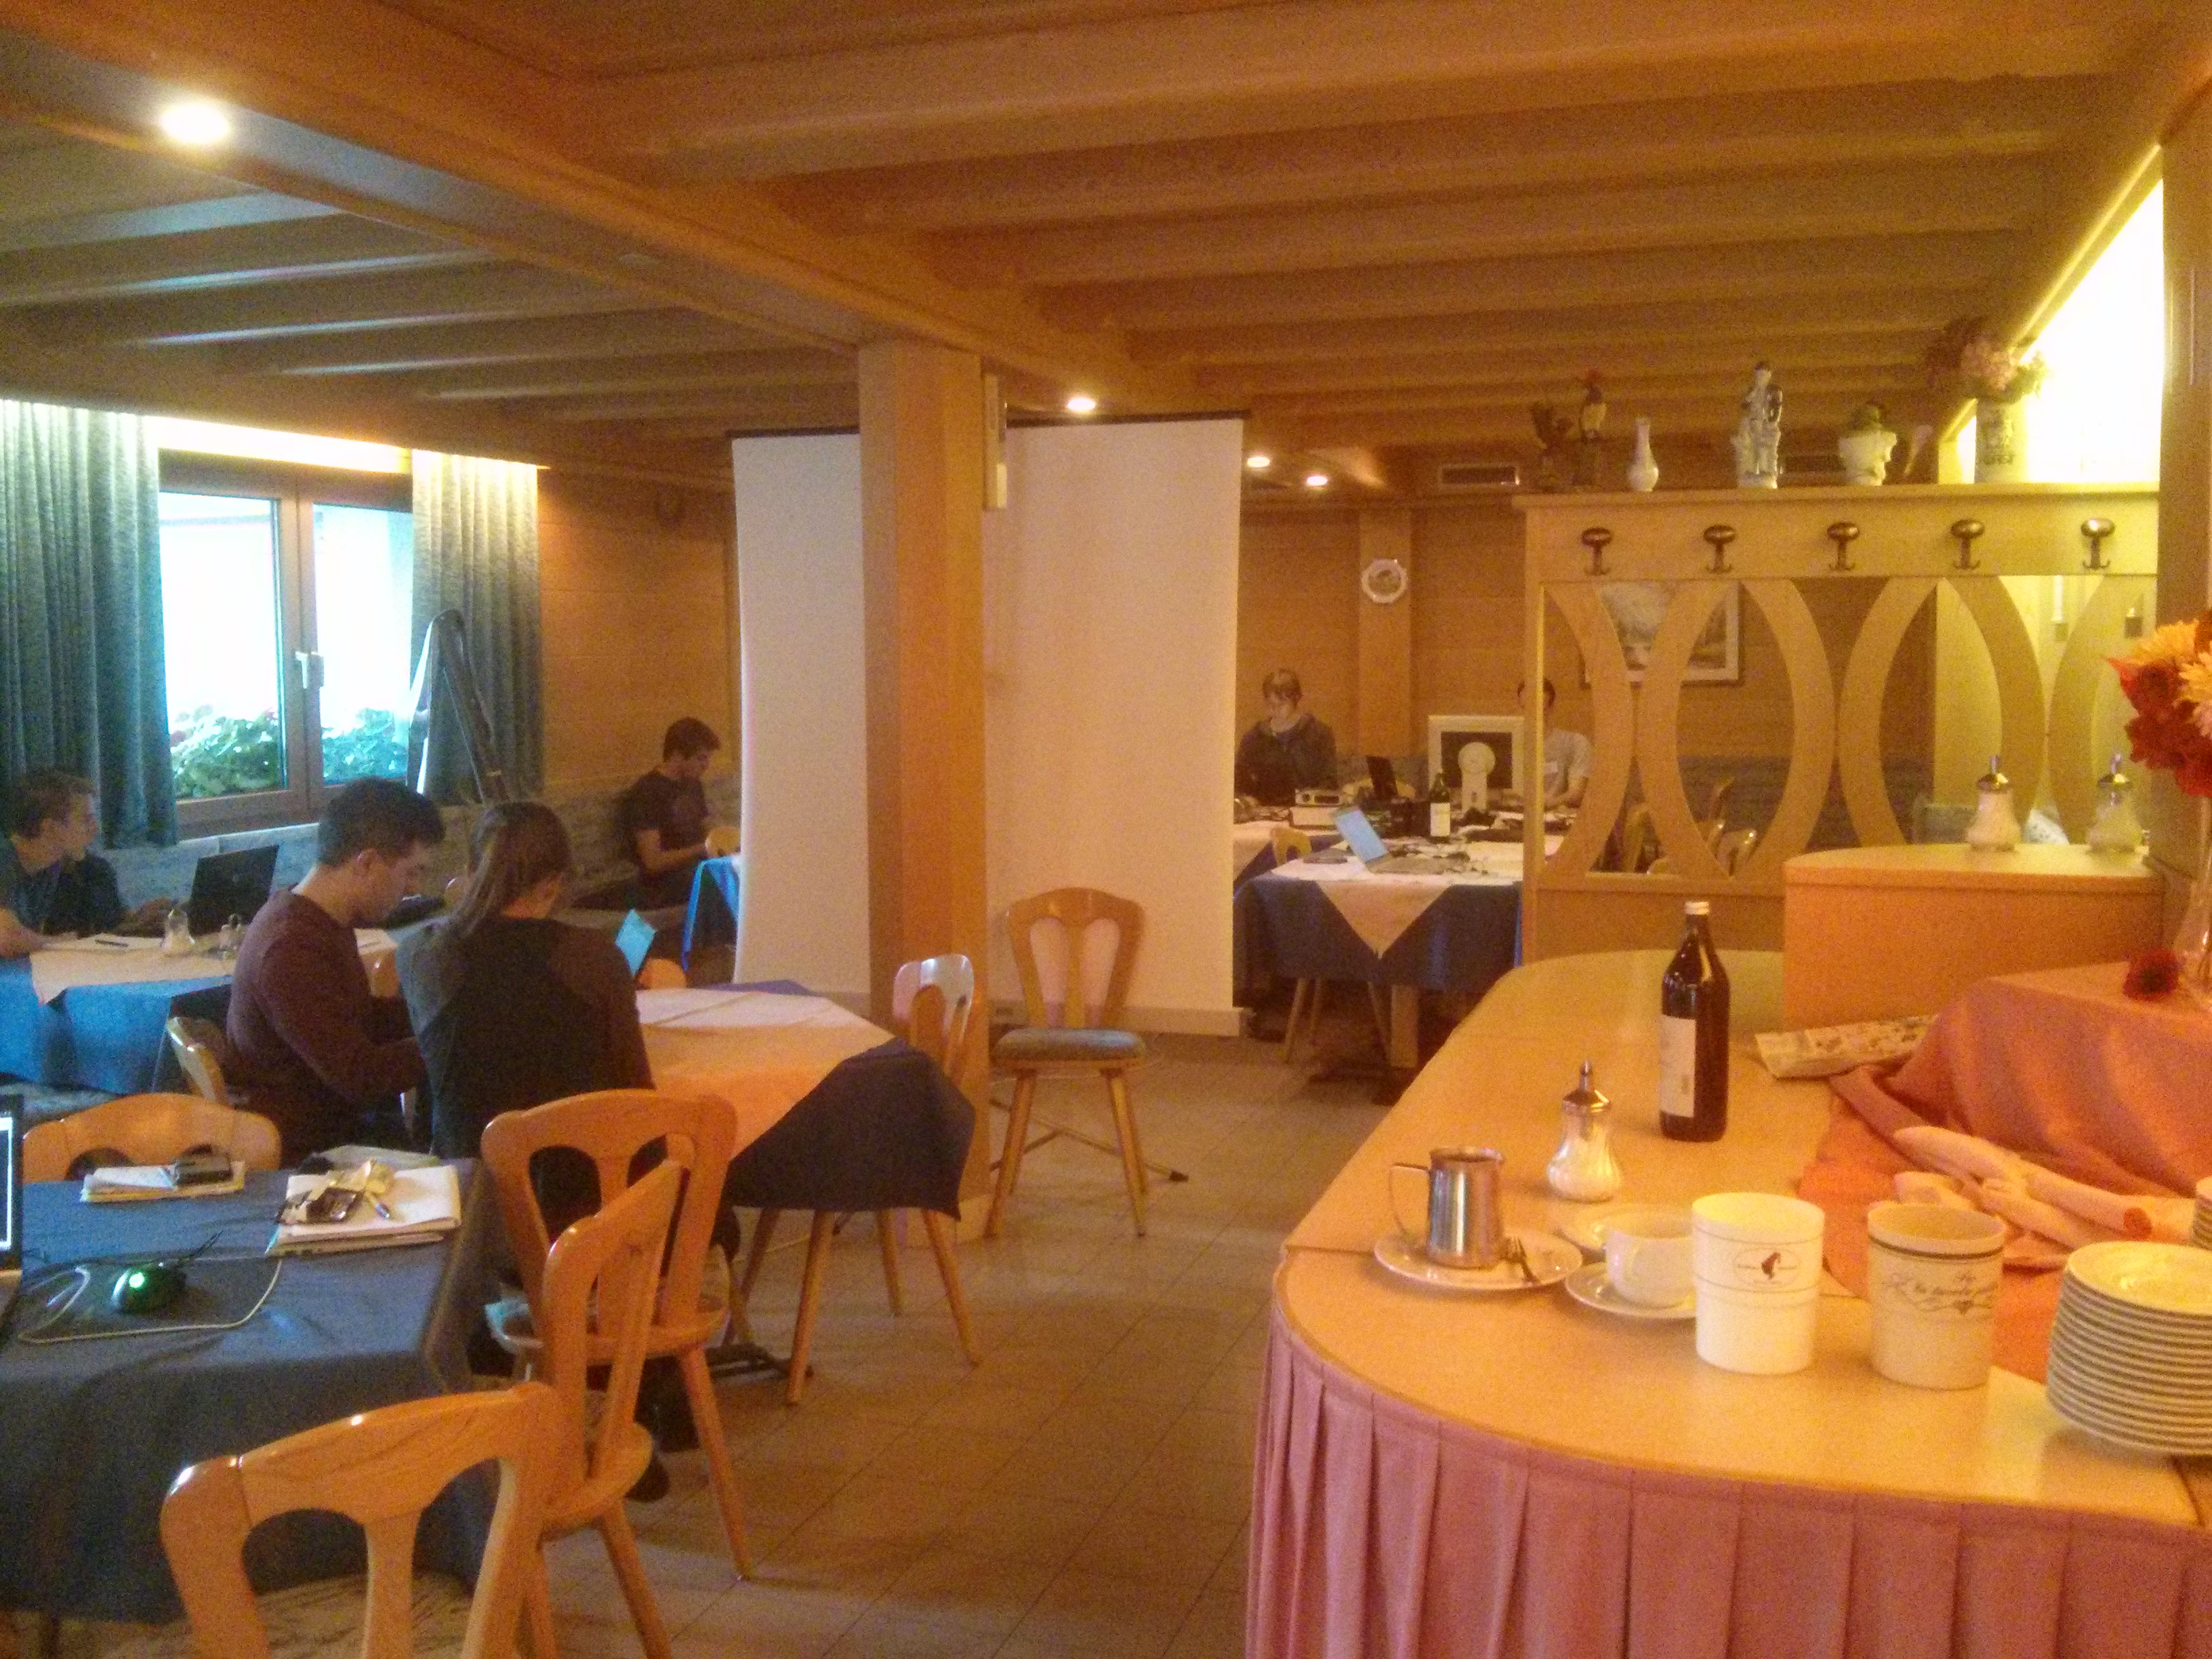
\includegraphics[scale=0.048]{img/Project.jpg}%
 		\caption{Students working on their project.}\label{fig:project}%
 	\end{center}%
\end{figure}

\begin{figure*}[ht]%
	\centering
    \begin{subfigure}[t]{0.5\textwidth}
 	\begin{center}%
 		\includegraphics[scale=0.05]{img/Hike1.jpg}%
 		%\caption{Presentation in a course.}\label{fig:hike1}%
 	\end{center}%
    \end{subfigure}%
    \begin{subfigure}[t]{0.5\textwidth}
 	\begin{center}%
 		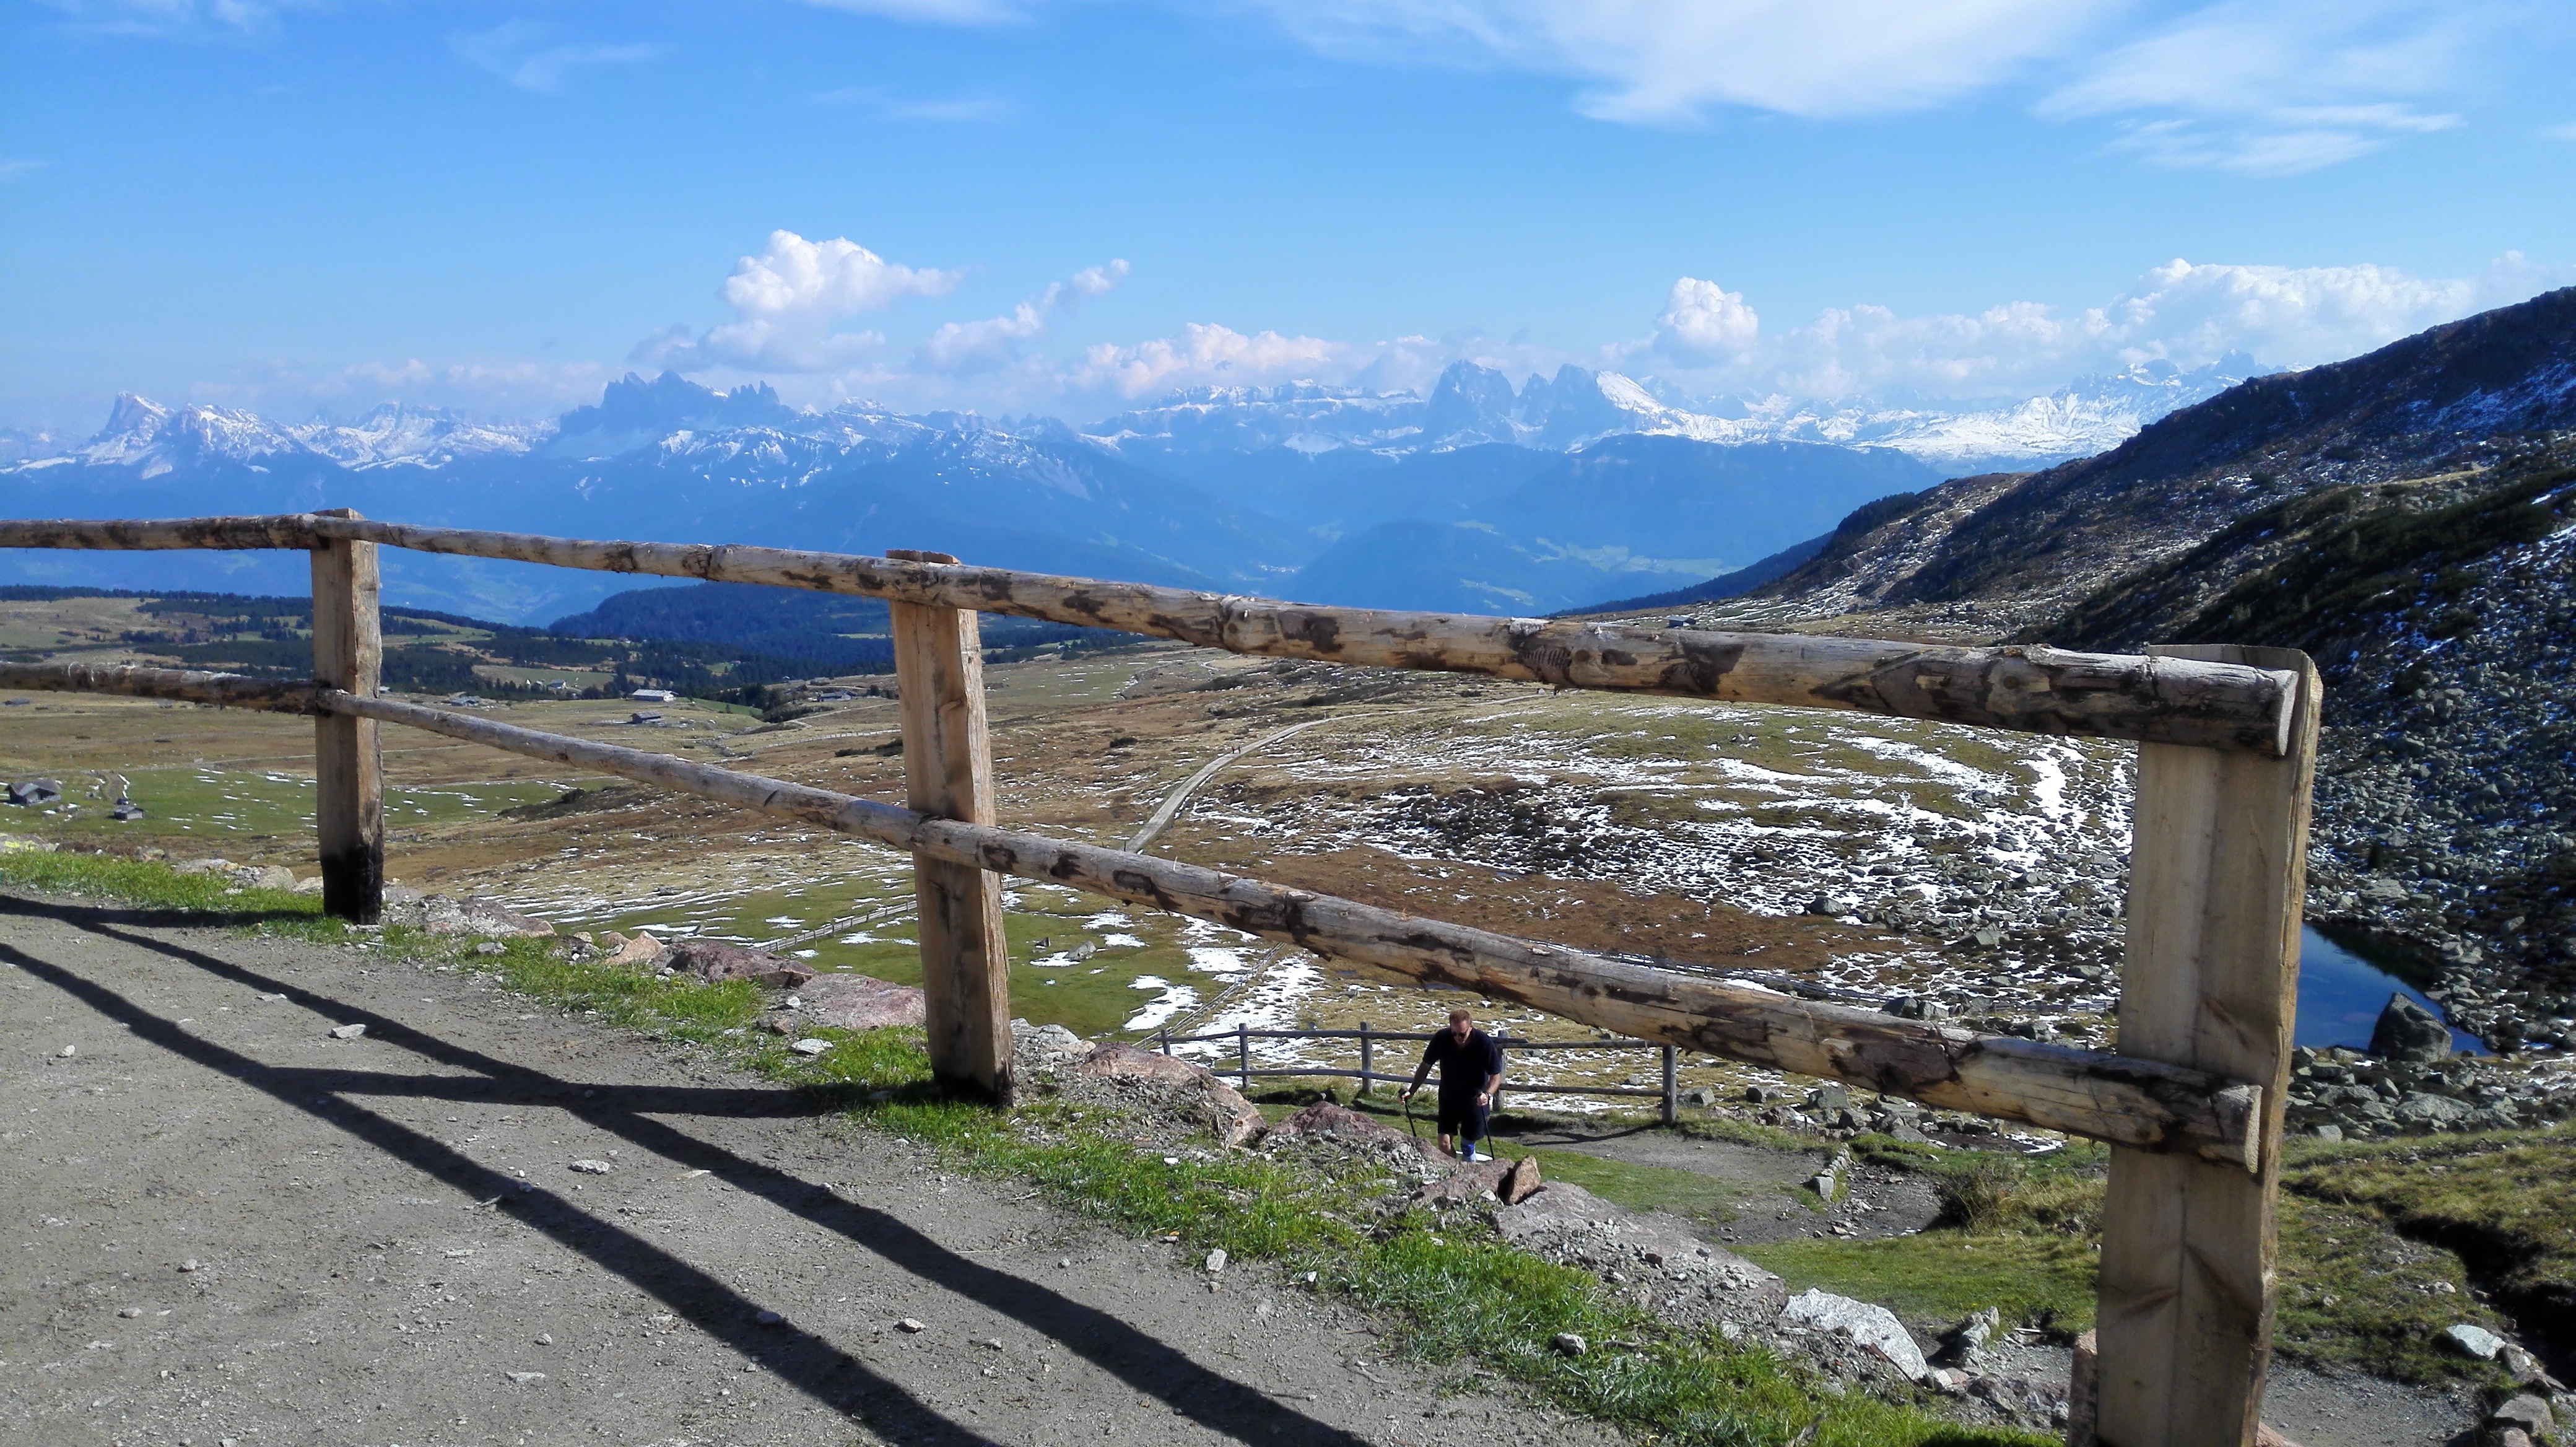
\includegraphics[scale=0.05]{img/Hike2.jpg}%
 		%\caption{Presentation in a course.}\label{fig:hike1}%
 	\end{center}%
    \end{subfigure}
    \caption{Impressions from hikes.}
    \label{fig:hiking}
\end{figure*}
\subsection{Hiking}
Right after the courses, the arguably second most important part of Ferienakademie is hiking. (Some people might even claim the hikes to be more important than the courses.) Sarntal and Southern Tyrol offer a beautiful landscape in the Alps and a variety of different hiking routes exist. While there are official hiking dys (also to make sure that some professors do not overwhelm their students), most of the courses also plan hiking trips on their own. There is even a competitiveness between different courses since on the final day, the cards are laid own the table and the course with the most hikes will be crowned (unofficially, admittedly, but there is still a lot of pride involved). But words can hardly describe the beauty of these trips, hence we refer to \autoref{fig:hiking}.

\subsection{Culture}
Of course, the cultural aspects of Sarntal play an important part at Ferienakademie as well. On one of the first days all participants meet up in a local town hall and get introduced to the history and culture of Sarntal. This evening is known as "Trldieaf" (how was that called again) which includes a presentation about the valley as well as traditional songs and clothing, see \autoref{fig:culture1}. Afterwards, one can enjoy the local wines (but be careful, it is not water!). 

Furthermore, a trip to Bolzano takes place, one of the big cities of South Tyrol, see \autoref{fig:culture2}. A highlight here is for example the South Tyrol Museum of Archaeology which features the Neolithic mummy "Ötzi".
\begin{figure}[ht]%
 	\begin{center}%
 		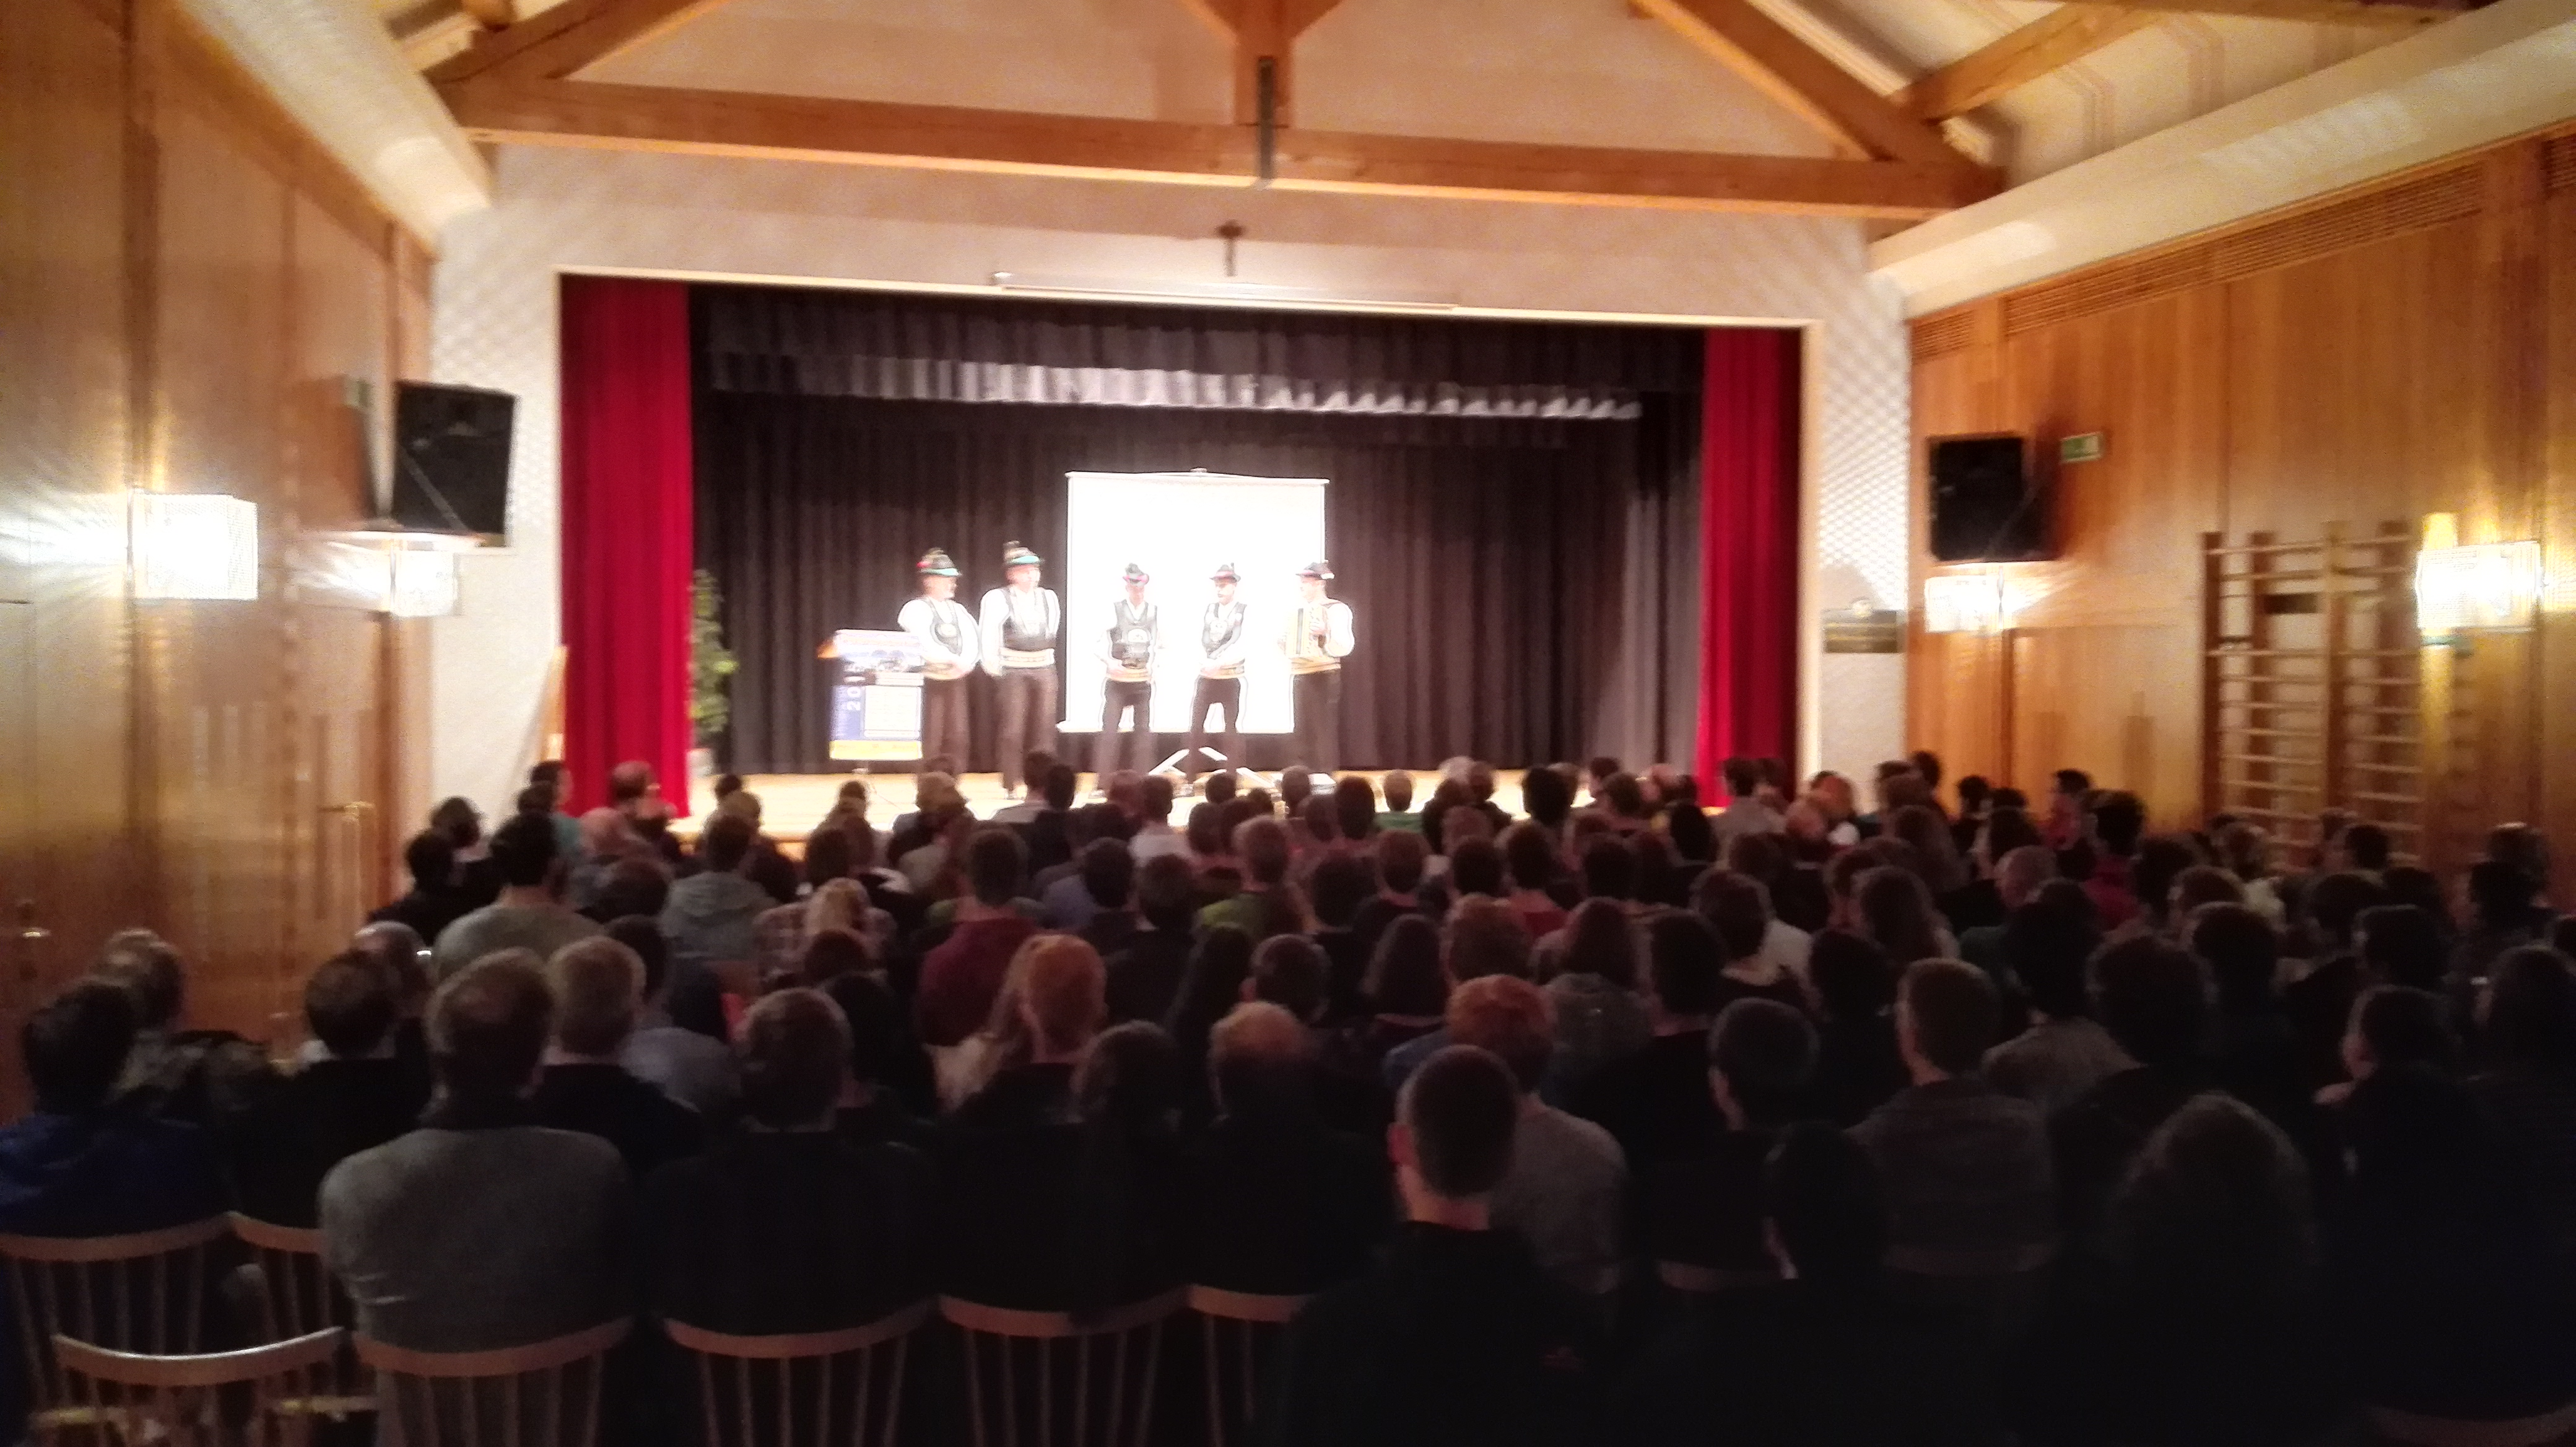
\includegraphics[scale=0.045]{img/Culture1.jpg}%
 		\caption{Trldiaf.}\label{fig:culture1}%
 	\end{center}%
\end{figure} 
\begin{figure}[ht]%
 	\begin{center}%
 		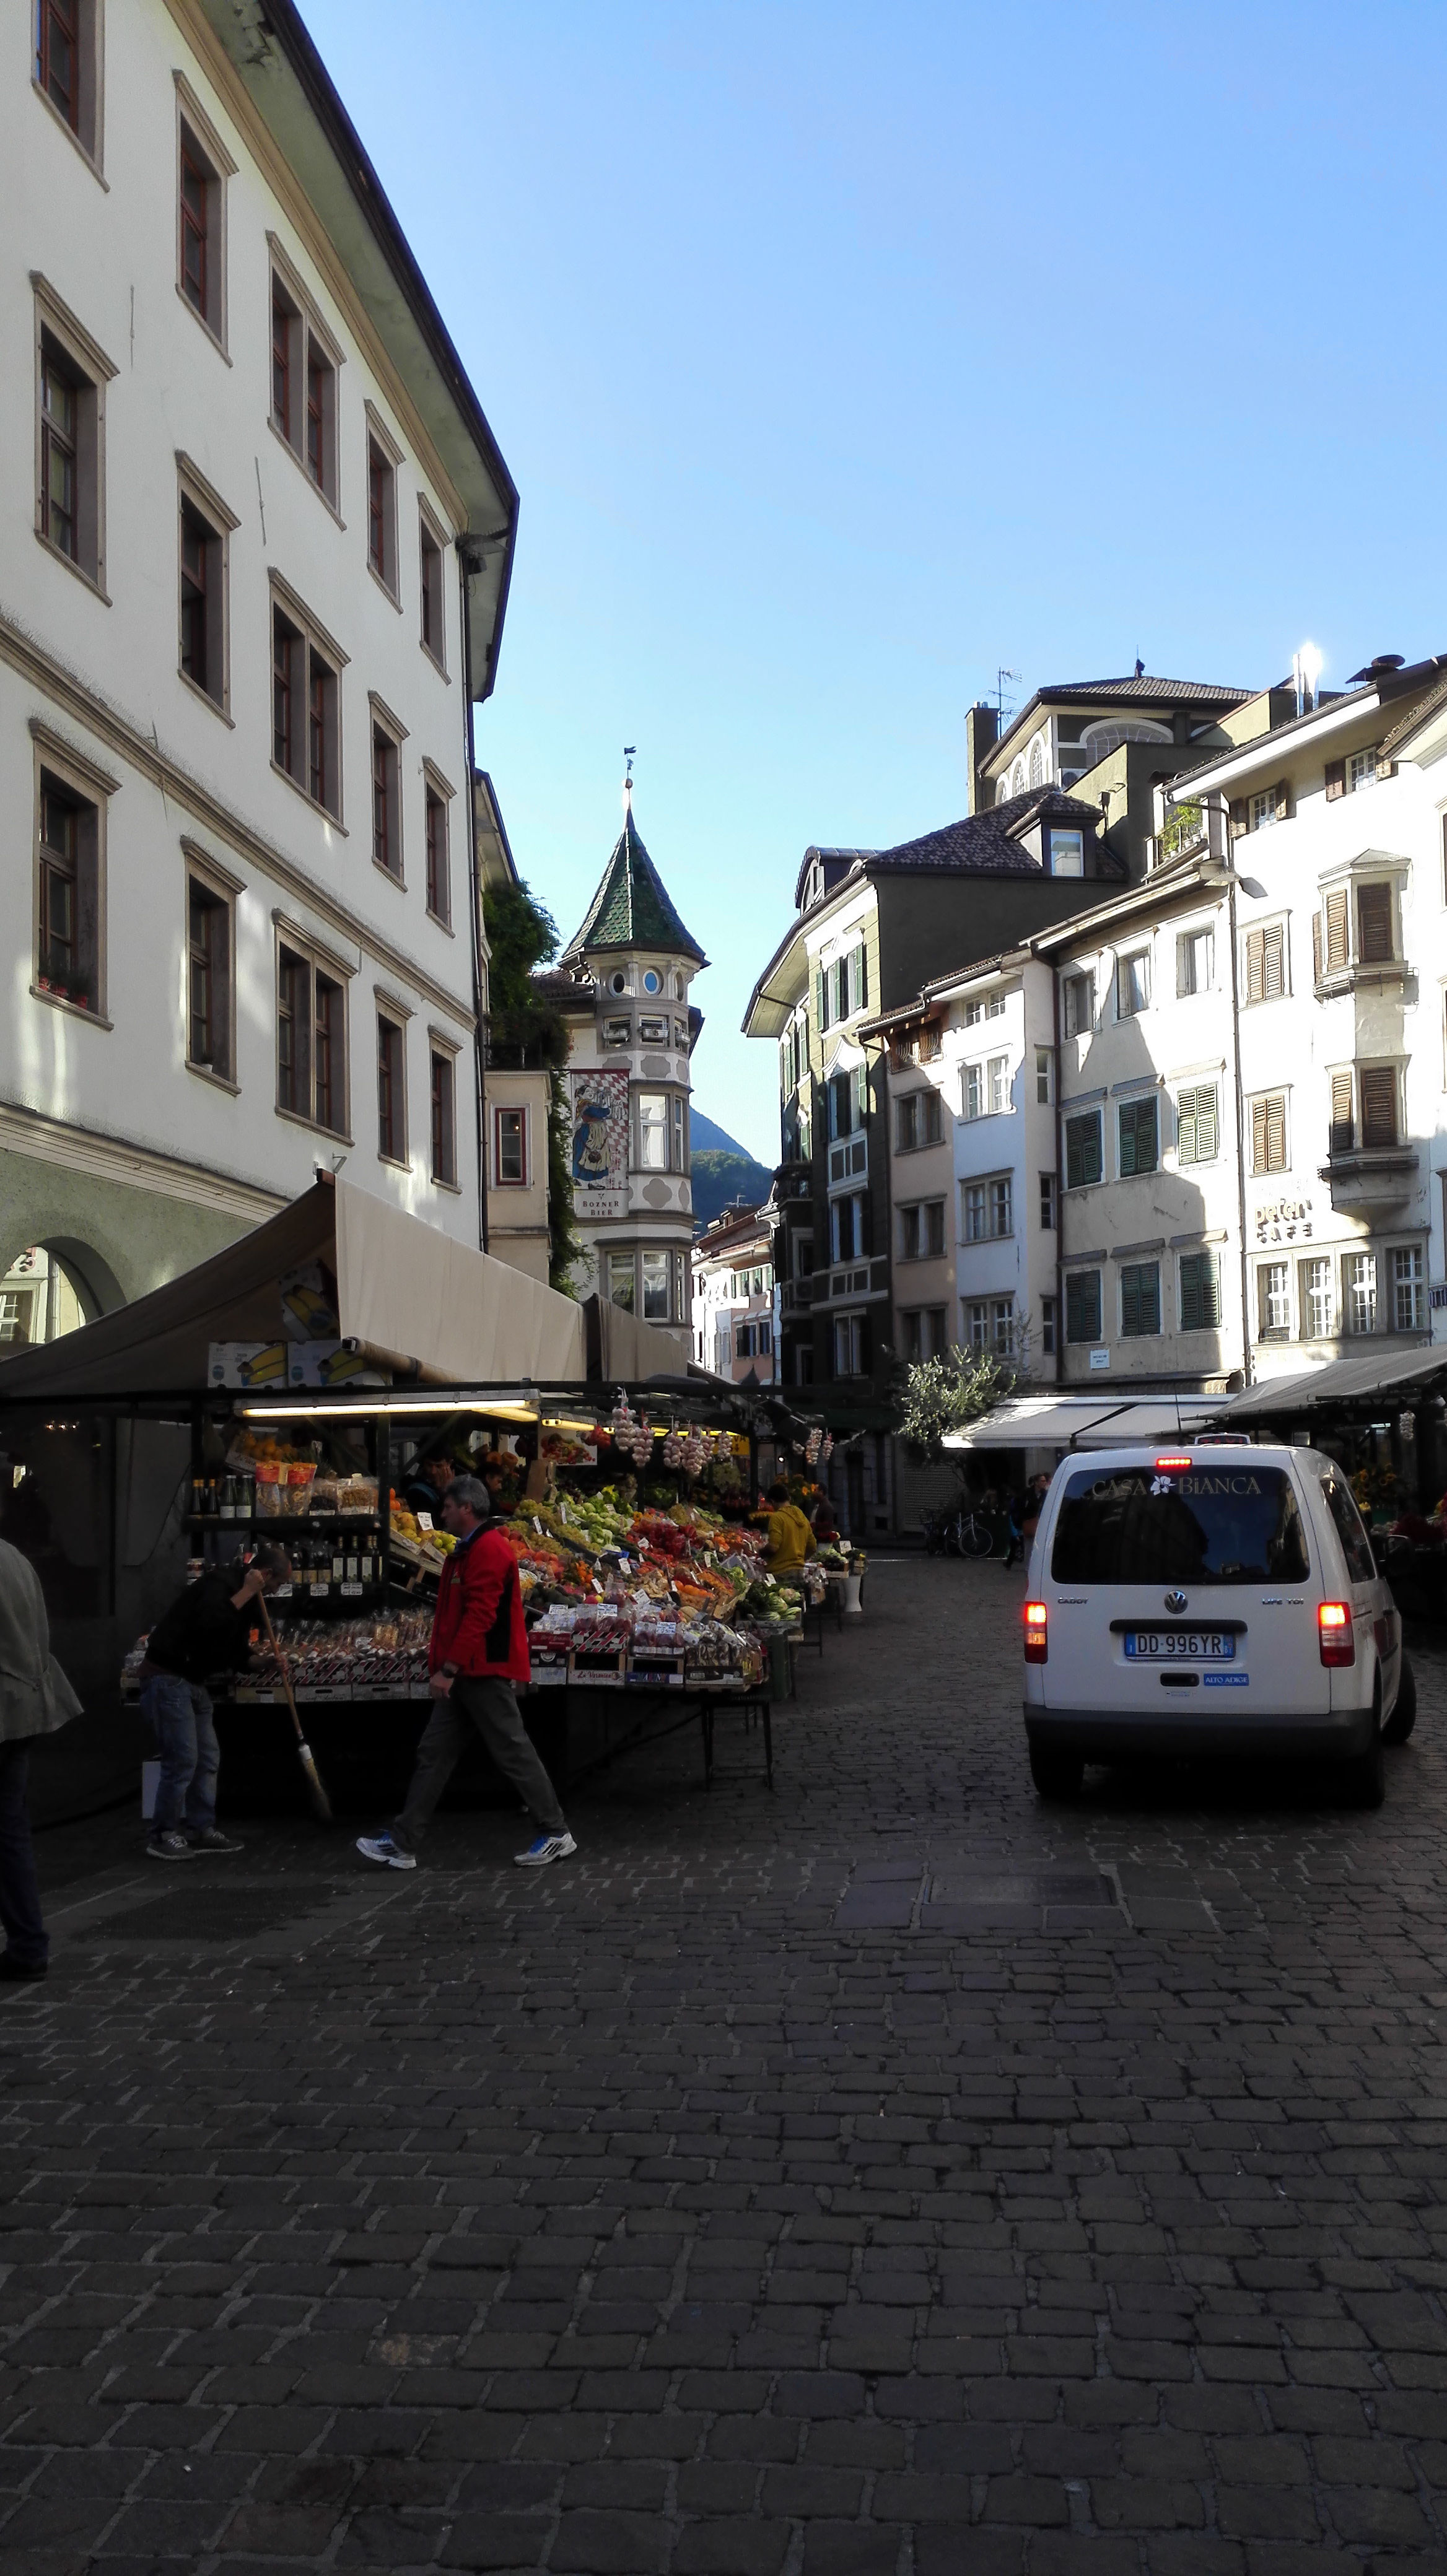
\includegraphics[scale=0.05]{img/Bolzano.jpg}%
 		\caption{Bolzano}\label{fig:culture2}%
 	\end{center}%
\end{figure} 

\subsection{Sport}
Each year three different competitions are offered where students can take part:
\begin{itemize}
\item Tabletennis
\item Chess
\item Run
\end{itemize}
Tabletennis and chess competitions are held as tournaments where each house puts together a team. The houses then compete against each other in semifinals and finals. For the tournament, each team brings their fans and their is always a great atmosphere during the games (of course not in chess)-- see \autoref{fig:Tabletennis}. 
\begin{figure}[ht]%
 	\begin{center}%
 		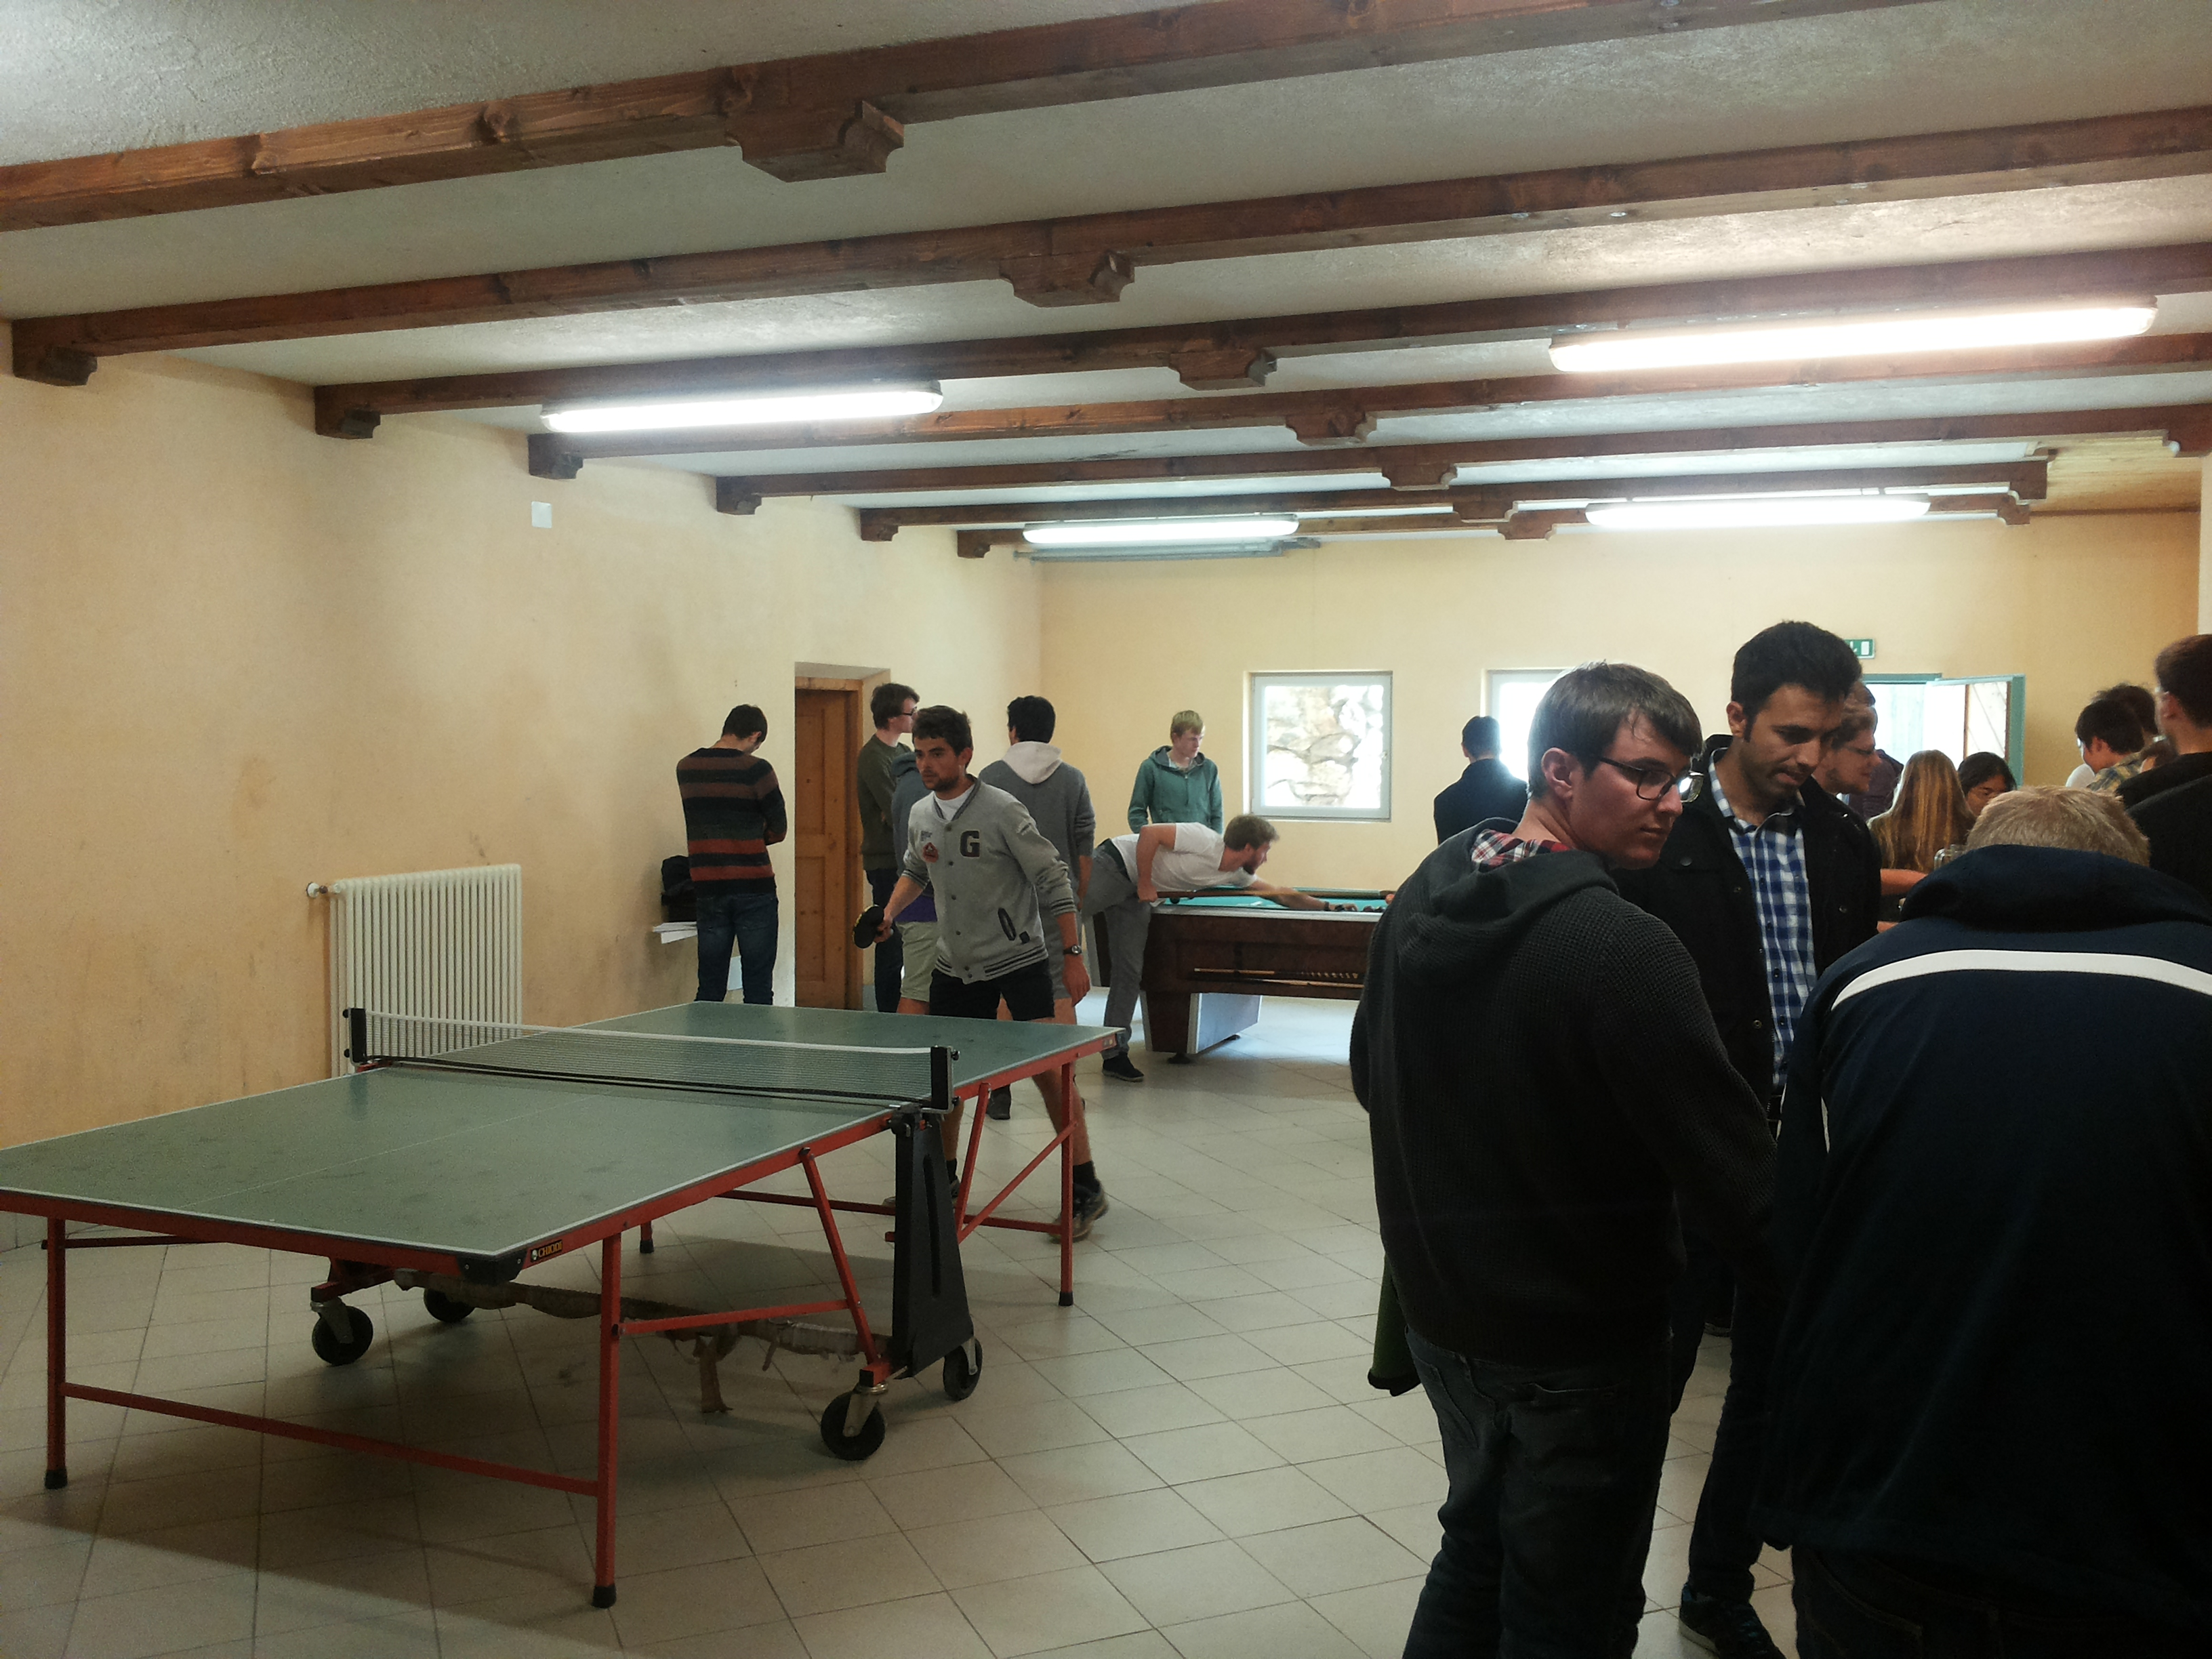
\includegraphics[scale=0.06]{img/Tabletennis.jpg}%
 		\caption{Preparing for the tabletennis tournament.}\label{fig:Tabletennis}%
 	\end{center}%
\end{figure}

The run is located at a beautiful spot, going around Lake Durnholz twice for about a total length of 4 km (????? check that) where the participants (and fans) can afterwards enjoy a refreshing swim in the lake. 

To show the importance of these activities, it is said, that some professors value the result of the tournaments higher than the results in the actual courses.

\subsection{Food}
Last but not least, the food. Although some courses hike more than 50 km [reference needed] and the rest of the time your brain needs every nutrition there is, nobody returns from Ferienakademie with a loss in weight. There is not only a variety of offers for food but also a lot! The choice might range from noodle buffet over dumpling buffet to schnitzel and Jause. And then there is Kaiserschmarrn. If you have never eaten Kaiserschmarrn wait till Ferienakademie. Not only is it mandatory to eat at every hut you take a break during hikes; there is also a special Kaiserschmarrn-evening where the students try to eat the kitchen empty-- literally. Prof. Bungartz likes to tell the story of Feldrand having to buy eggs from a neighbouring farm to provide more Kaiserschmarrn for the hungry students. How beautiful and delicious a Kaiserschmarrn simply can look is illustrated in \autoref{fig:Kaiserschmarrn}.
\begin{figure}[ht]%
 	\begin{center}%
 		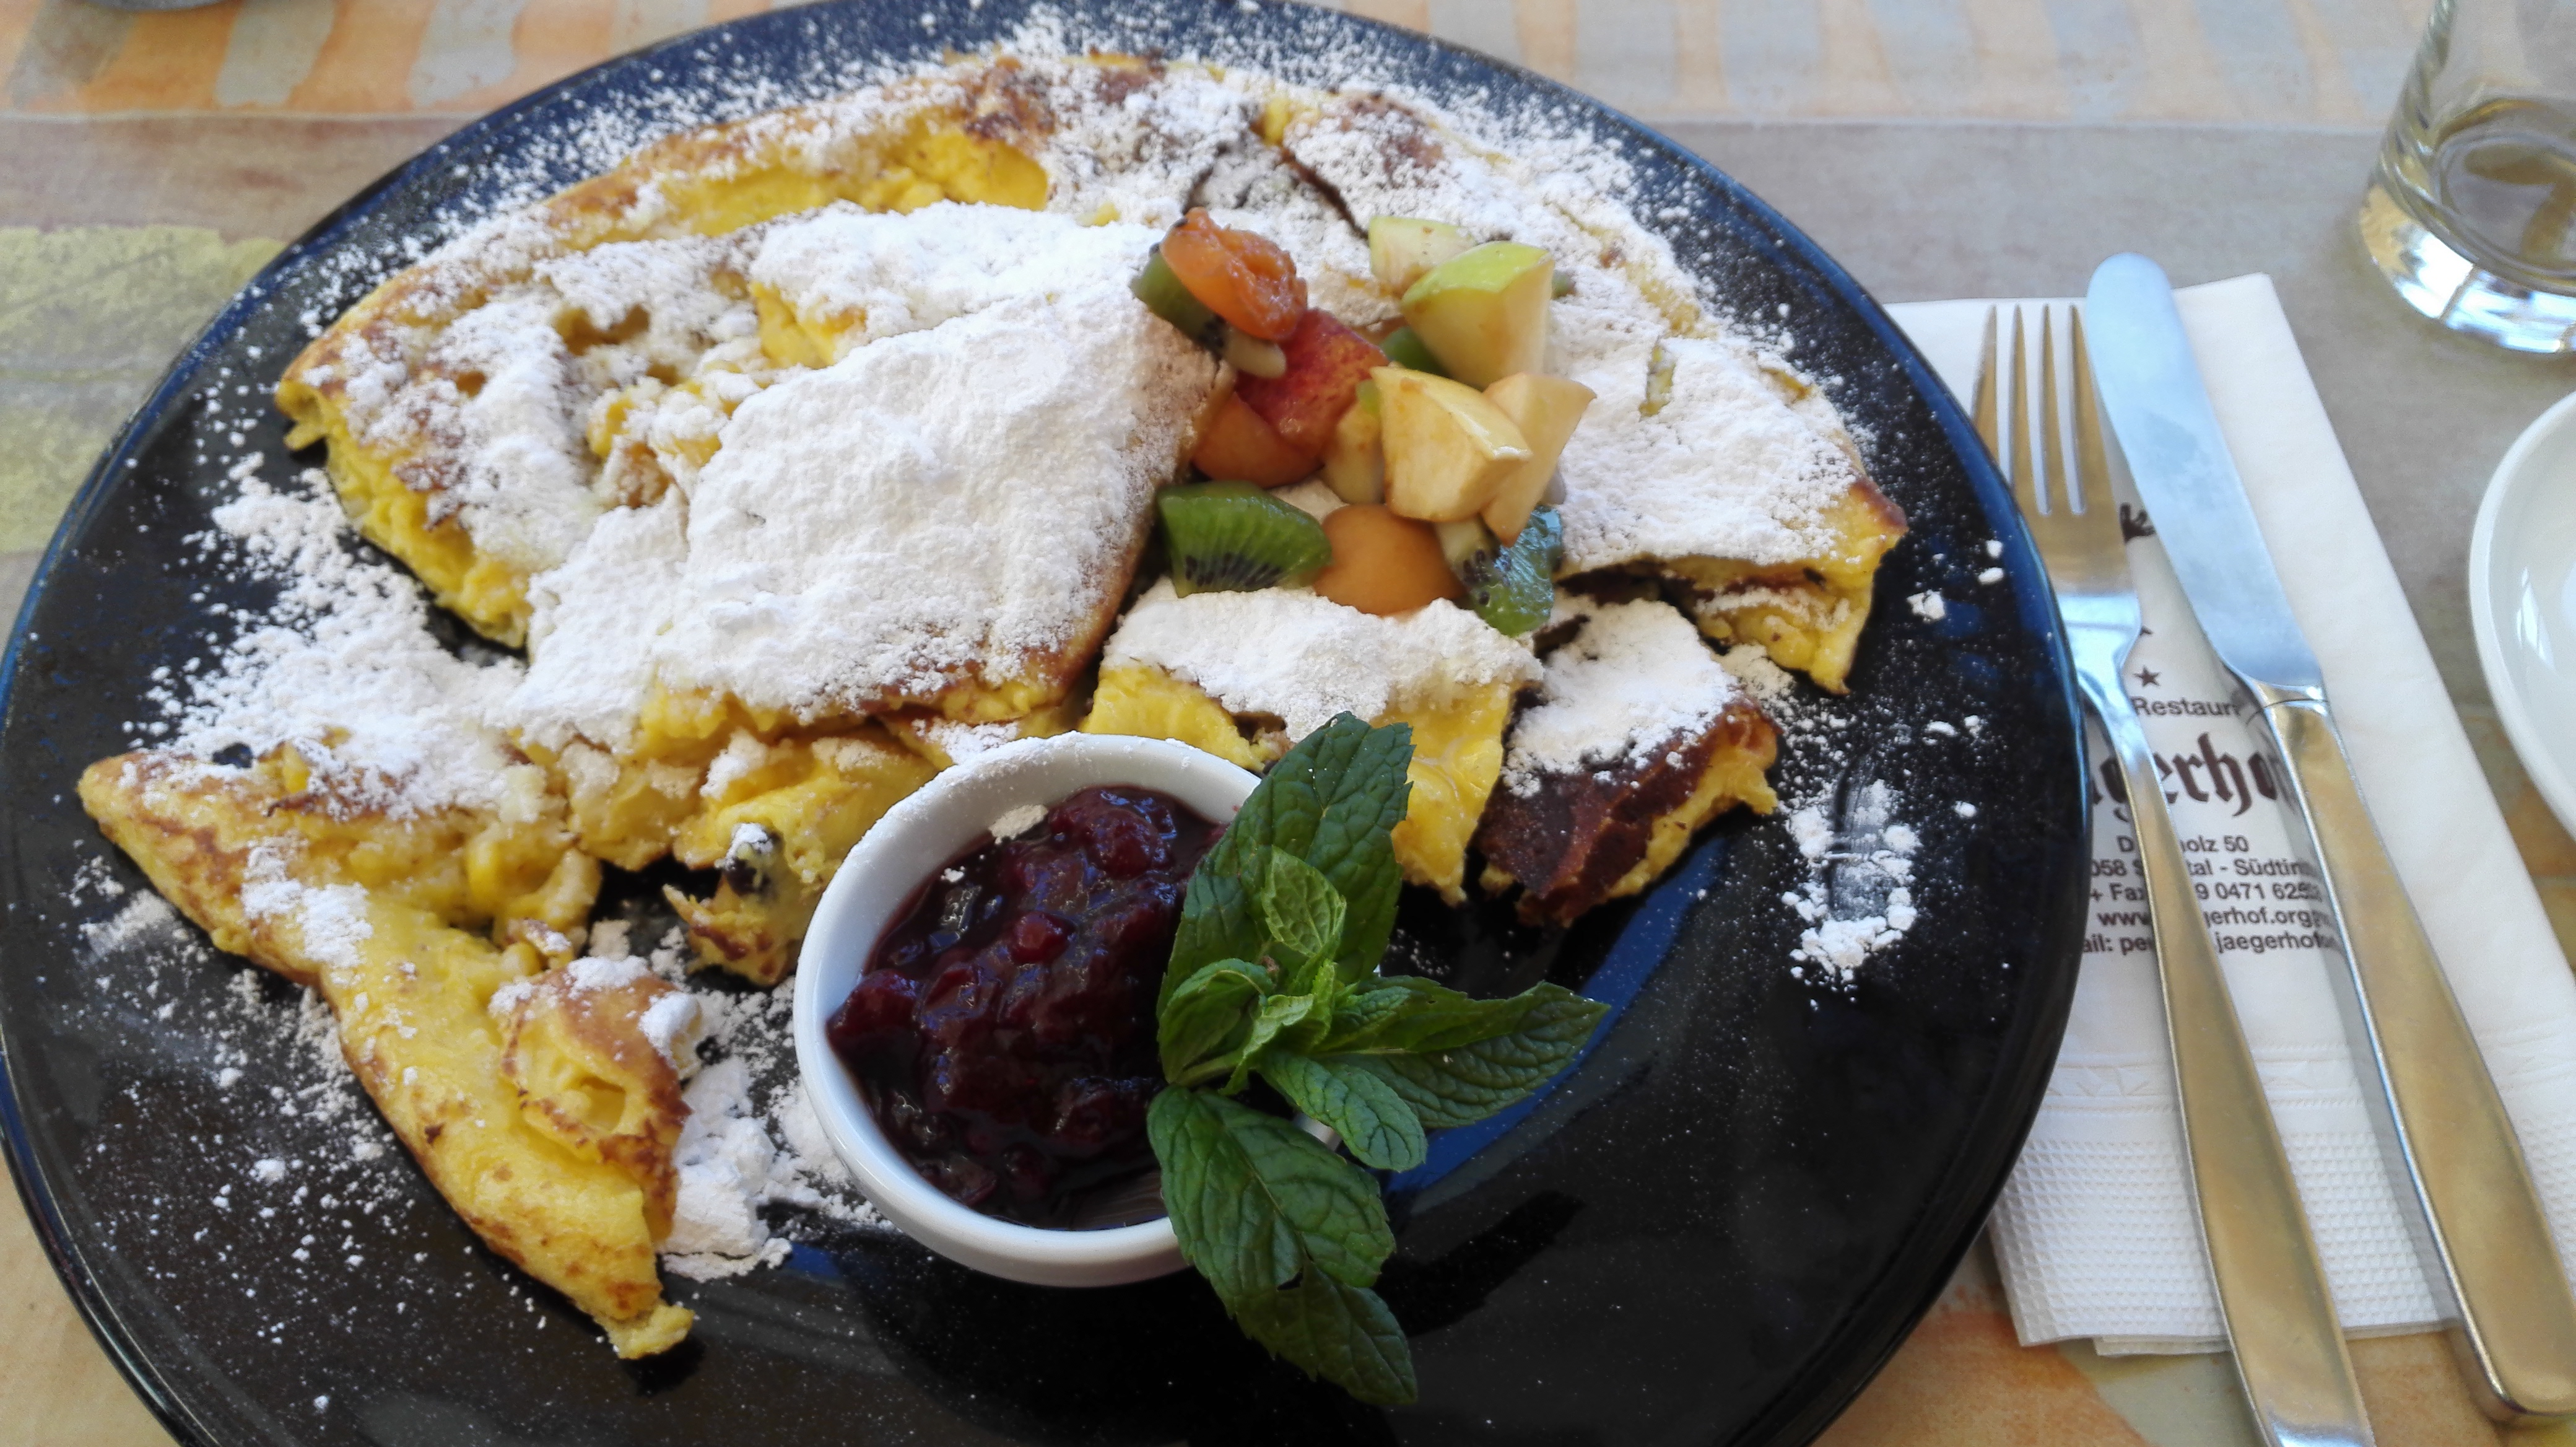
\includegraphics[scale=0.05]{img/Kaiserschmarrn.jpg}%
 		\caption{Kaiserschmarrn [Jägerhof et al.]}\label{fig:Kaiserschmarrn}%
 	\end{center}%
\end{figure}

During our stay at Ferienakademie a love for Kaiserschmarrn has itself developed which we would like to express by the following poem-- Ode an den Kaiserschmarrn (with the rhythm of Friedrich Schiller's "Ode an die Freude"). 
\begin{figure}[ht]
\begin{framed}
An den Kaiserschmarrn 
\\
\\
%\begin{small}
Freude, leck'rer Kaiserschmarren,\\
Mehlspeis mit Rosinen,\\
Wir verspeisen wie Barbaren \\
hunderte Portionen.\\

Jede Wand'rung endet wieder \\
mit nem Blech voll Kaiserschmarrn.\\
Studenten, die am meisten essen,\\
die sieht Bungartz voll stolz an.
%\end{small}
\end{framed}
\end{figure}
\vfill
%\columnbreak